\input{../preamble}

\author{Niccolò Nicolosi}
\institute{Politecnico di Milano}
\date{2025/2026}
\title{MLIR}
\subtitle{Multi-Level Intermediate Representation}
\newcommand{\customdata}{Niccolò Nicolosi}

\AtBeginSection[]
{
\begin{frame}{Contents}
\tableofcontents[currentsection]
\end{frame}
}


\begin{document}


\begin{frame}
\maketitle
\end{frame}


\begin{frame}{Lecture Outline}
\tableofcontents
\end{frame}


% ─────────────────────────────────────────────────────────────────────────────
\section{Introduction \& Motivation}


\begin{frame}{Recap: LLVM}
  LLVM is a compiler framework built around a single, unified IR:
  \medskip

  \textbf{\textcolor{mainAccent}{LLVM-IR: a low-level, RISC-like, SSA-based representation}}

  \bigskip
  \begin{center}
    \vspace{-.05\textheight}
    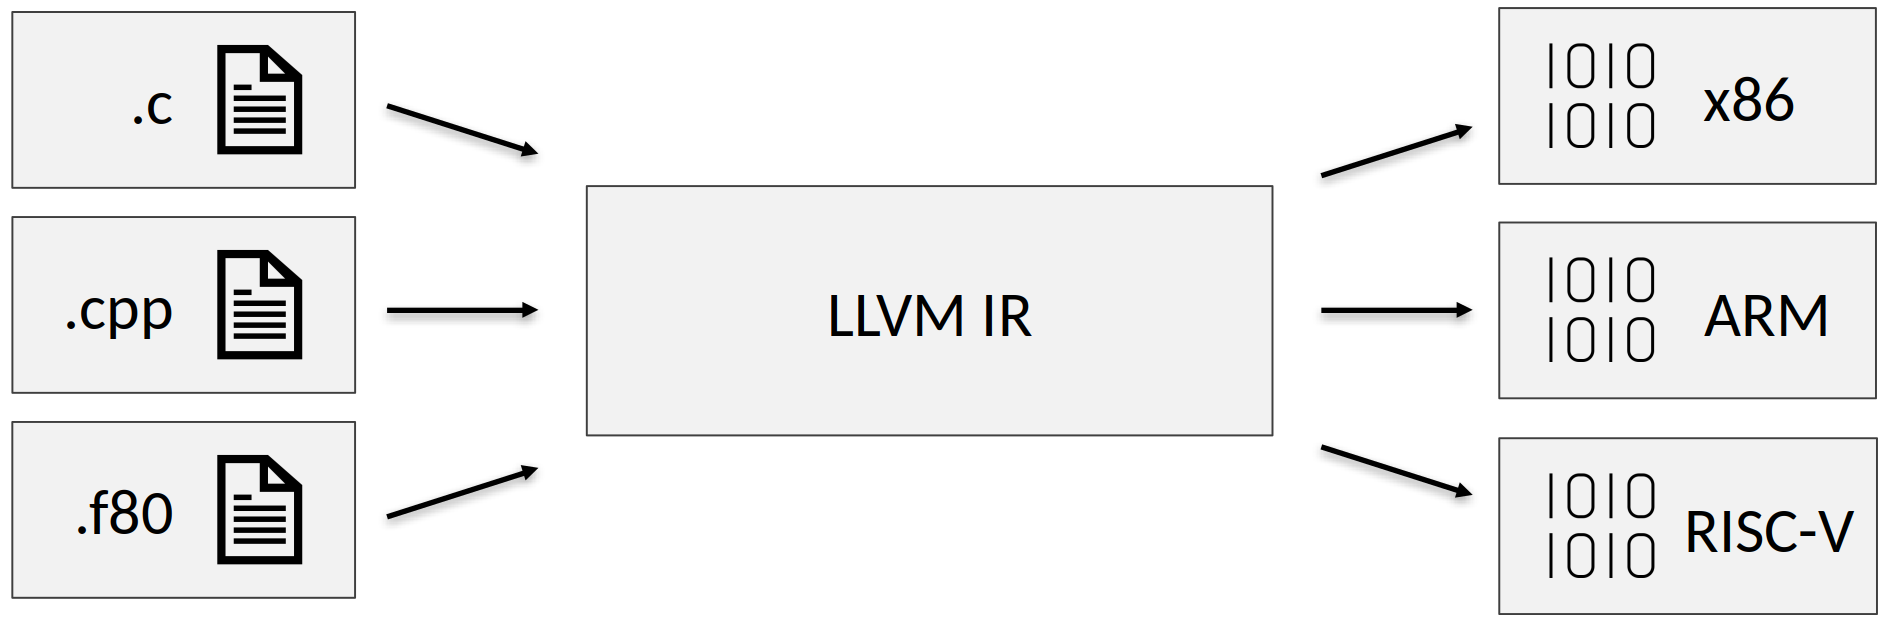
\includegraphics[width=\textwidth]{img/llvm.png}
  \end{center}
\end{frame}


\begin{frame}{LLVM-IR Limitations}
  LLVM-IR is a great target IR, but poor for high-level
  optimizations:
  \bigskip
  \begin{itemize}
    \item Too low-level
    \item No practical notion of loops, arrays, or linear algebra
    \item No notion of hardware accelerators (GPUs, FPGAs, NPUs)
  \end{itemize}
  \bigskip
  \textbf{\textcolor{mainAccent}{Lowering to LLVM-IR destroys high-level structure
  irreversibly}}
\end{frame}


\begin{frame}{The Domain-Specific Compiler Problem}
  Before MLIR, every domain invented its own IR\ldots

  \bigskip
  \begin{columns}
    \begin{column}{0.48\textwidth}
      \begin{block}{ML frameworks}
        TensorFlow XLA, TFLite, Torch IR, ONNX\ldots
      \end{block}
      \medskip
      \begin{block}{Hardware synthesis}
        CIRCT FIRRTL, HLS pragmas\ldots
      \end{block}
    \end{column}
    \begin{column}{0.48\textwidth}
      \begin{exampleblock}{HPC / polyhedral}
        Polly, Pluto, OpenScop\ldots
      \end{exampleblock}
      \medskip
      \begin{exampleblock}{Quantum}
        QIR, OpenQASM\ldots
      \end{exampleblock}
    \end{column}
  \end{columns}

  \bigskip
  \begin{center}
    \textbf{\textcolor{mainAccent}{%
      Duplicated effort, no interoperability, no shared tooling}}
  \end{center}
\end{frame}


\begin{frame}{What is MLIR?}
  \textbf{MLIR = Multi-Level Intermediate Representation}\\
  \textit{\small A sub-project of LLVM (since 2019, originally from Google)}

  \bigskip
  \begin{itemize}
    \item \textbf{A framework for building compiler IRs}
      \begin{itemize}
        \item Designed to support multiple abstraction levels simultaneously
      \end{itemize}
    \item \textbf{A toolbox covering typical compiler infrastructure needs}
      \begin{itemize}
        \item Diagnostics, pass infrastructure, multi-threading, testing, \ldots
      \end{itemize}
    \item \textbf{An extensible and composable ecosystem of IRs (dialects)}
      \begin{itemize}
        \item Different IRs can coexist in the same program
        \item Progressive lowering from high-level to low-level
      \end{itemize}
  \end{itemize}
\end{frame}


\begin{frame}{What MLIR is NOT}
  \begin{block}{NOT a language}
    MLIR is not a fixed IR with fixed semantics.\\
    It is an extensible framework to define IRs.
  \end{block}
  \medskip
  \begin{exampleblock}{NOT a compiler}
    MLIR does not compile anything by itself.\\
    It is a framework for building compilers.
  \end{exampleblock}
  \medskip
  \begin{block}{NOT Machine Learning IR}
    Despite the acronym, MLIR is a general-purpose\\
    compiler infrastructure used across many domains.
  \end{block}
\end{frame}


\begin{frame}{MLIR in the LLVM Ecosystem}
  \begin{center}
  \begin{tikzpicture}[
    enode/.style={rectangle, fill=exampleAccent, text=white,
                  font=\small\bfseries, text width=2.15cm,
                  minimum height=1.0cm, align=center},
    mnode/.style={rectangle, fill=mainAccent, text=white,
                  font=\small\bfseries, text width=2.15cm,
                  minimum height=1.0cm, align=center}]
    \node[enode] (src)  at (0.0, 0.0)  {Source\\Code};
    \node[mnode] (fe)   at (2.8, 0.0)  {Frontend};
    \node[mnode] (mlir) at (5.6, 0.0)  {MLIR\\Dialects};

    \node[mnode] (ir)   at (5.6,-1.9)  {LLVM\\Middle-end};
    \node[mnode] (be)   at (2.8,-1.9)  {LLVM\\Backend};
    \node[enode] (mc)   at (0.0,-1.9)  {Machine\\Code};

    \draw[->, thick, gray] (src.east) -- (fe.west);
    \draw[->, thick, gray] (fe.east) -- (mlir.west);
    \draw[->, thick, gray] (mlir.south) -- (ir.north);
    \draw[->, thick, gray] (ir.west) -- (be.east);
    \draw[->, thick, gray] (be.west) -- (mc.east);
  \end{tikzpicture}
  \end{center}
  \bigskip
  \begin{itemize}
    \item \textbf{MLIR sits between the frontend and LLVM-IR}
      \begin{itemize}
        \item Enables multi-level, progressive transformations
        \item Can also target hardware directly (bypassing LLVM)
      \end{itemize}
    \item MLIR can lower to LLVM-IR via the
          \textbf{\textcolor{mainAccent}{\texttt{llvm} dialect}}
  \end{itemize}
\end{frame}


% ─────────────────────────────────────────────────────────────────────────────
\section{MLIR Core Concepts}


\begin{frame}{Operations}
  \framesubtitle{The Basic Building Block}
  In MLIR, everything is an \textbf{\textcolor{mainAccent}{Operation}} (Op).\\
  \textit{\small Ops are the generalization of LLVM Instructions, but far more powerful.}

  \bigskip
  \begin{itemize}
    \item \textbf{An Op has a unique name (\texttt{dialect.opname})}
      \begin{itemize}
        \item \texttt{\textcolor{mainAccent}{%
              func.call,\ \ arith.addi,\ \ linalg.matmul,\ \ scf.for}}
      \end{itemize}
    \item \textbf{Zero or more SSA operands} (inputs)
    \item \textbf{Zero or more SSA results} (outputs, each with a type)
    \item \textbf{A dictionary of Attributes} (compile-time constant metadata)
    \item \textbf{Zero or more Regions} (for structured control flow)
    \item Source location for diagnostics
  \end{itemize}
\end{frame}


\begin{frame}[fragile]{Operations}
  \framesubtitle{Textual Syntax}
  Every Op can be written in a universal generic form:
\begin{lstlisting}[language=none,basicstyle=\ttfamily\small]
%result = "dialect.op_name"(%arg0, %arg1)
            {attr_name = value : attr_type}
            : (operand_type0, operand_type1)
            -> result_type
\end{lstlisting}

  Dialects may define a custom syntax (assembly format). Examples:
\begin{lstlisting}[language=none,basicstyle=\ttfamily\small]
// generic form:
%0 = "arith.addi"(%a, %b) : (i32, i32) -> i32
// custom form:
%0 = arith.addi %a, %b : i32

// assembly format of a function:
func.func @add(%a: i32, %b: i32) -> i32 {
  %r = arith.addi %a, %b : i32
  func.return %r : i32
}
\end{lstlisting}
\end{frame}


\begin{frame}[fragile]{Values}
  \textbf{\textcolor{mainAccent}{Values}} are the SSA objects that flow between operations.

  \bigskip
  \begin{itemize}
    \item A value is either:
      \begin{itemize}
        \item an \textbf{Op result}, produced by an operation
        \item a \textbf{Block argument}, introduced at block entry
      \end{itemize}
    \item Values are the data; Operations define the semantics
  \end{itemize}

\begin{lstlisting}[language=none,basicstyle=\ttfamily\small]
func.func @add_mul(%a: i32, %b: i32, %c: i32) -> i32 {
  %sum = arith.addi %a, %b : i32   // Op result value
  %res = arith.muli %sum, %c : i32 // Uses previous value
  func.return %res : i32
}
\end{lstlisting}

\end{frame}


\begin{frame}{Types in MLIR}
  MLIR is strongly typed. Every value has exactly one type.

  \medskip
  \begin{columns}
    \begin{column}{0.48\textwidth}
      \begin{block}{Built-in scalar types}
        \begin{itemize}
          \item \texttt{i1, i8, i16, i32,} \ldots
          \item \texttt{f16, f32, f64, bf16,} \ldots
          \item \texttt{index} {\small(platform-size integer)}
          \item \ldots
        \end{itemize}
      \end{block}
    \end{column}
    \begin{column}{0.48\textwidth}
      \begin{exampleblock}{Aggregate types}
        \begin{itemize}
          \item \texttt{tensor<4x4xf32>}
          \item \texttt{memref<4x4xf32>} {\small(buffer)}
          \item \texttt{vector<8xf32>} {\small(SIMD)}
          \item \ldots
        \end{itemize}
      \end{exampleblock}
    \end{column}
  \end{columns}

  \medskip
  \begin{block}{Dialect-defined types \hfill (extensible!)}
    \begin{itemize}
      \item Dialects may define entirely new types
      \item E.g.\ \texttt{llvm.ptr}, \texttt{llvm.struct<...>}\ldots
    \end{itemize}
  \end{block}
\end{frame}


\begin{frame}[fragile]{Attributes in MLIR}
  Attributes carry \textbf{\textcolor{mainAccent}{compile-time constant}} metadata on Ops.

\begin{lstlisting}[language=none,basicstyle=\ttfamily\small]
// integer attribute
%c42 = arith.constant 42 : i32 // {value = 42 : i32}

// string attribute (e.g. function linkage)
func.func @main() -> i32
  attributes {sym_visibility = "public"}

// dense array attribute
%cst = arith.constant dense<[1.0, 2.0, 3.0]> : tensor<3xf32>
\end{lstlisting}

  \begin{itemize}
    \item Attributes are immutable and uniqued by the \texttt{MLIRContext}
    \item Dialects can define custom attribute types
    \item Examples: integer, float, string, array, \ldots
  \end{itemize}
\end{frame}


\begin{frame}{Dialects}
  \begin{quote}
    ``A dialect is a grouping of functionality which can be used to extend the
    MLIR system.''
  \end{quote}

  \begin{block}{A dialect bundles together}
    \begin{itemize}
      \item \textbf{Operations}: the "instructions" of this IR level
      \item \textbf{Types}: new data types specific to this domain
      \item \textbf{Attributes}: compile-time metadata specific to this domain
      \item \textbf{Interfaces}: generic interaction hooks
      \item \textbf{Passes}: analyses or transformations acting on this dialect
    \end{itemize}
  \end{block}

  \bigskip
  Dialects are the \textbf{\textcolor{mainAccent}{primary extension mechanism}} of MLIR.\\
  They can be mixed within the same program.
\end{frame}


\begin{frame}[fragile]{Dialects}
  \framesubtitle{Co-existence in the Same IR}
  Multiple dialects can coexist in the same function.\\
  This is the key to progressive lowering:

\begin{lstlisting}[language=none,basicstyle=\ttfamily\small]
// After partial lowering:
// - Already lowered to func and arith
// - linalg.matmul is still high-level (not yet lowered)
func.func @matmul(%A: memref<4x4xf32>,
                  %B: memref<4x4xf32>,
                  %C: memref<4x4xf32>) {
  linalg.matmul
    ins(%A, %B : memref<4x4xf32>, memref<4x4xf32>)
    outs(%C : memref<4x4xf32>)
  func.return
}
\end{lstlisting}

  \textbf{\textcolor{mainAccent}{%
    High-level semantics preserved as long as needed.}}
\end{frame}


\begin{frame}[fragile]{Blocks}
  A \textbf{\textcolor{mainAccent}{Block}} is analogous to a Basic Block in LLVM-IR.

  \begin{itemize}
    \item A sequence of Ops executed in order
    \item Ends with a terminator Op (branch, return, yield\ldots)
    \item \textbf{Has zero or more Block Arguments (replace phi-nodes!)}
      \begin{itemize}
        \item In LLVM-IR: phi instructions \; In MLIR: block arguments
      \end{itemize}
  \end{itemize}

\begin{lstlisting}[language=none,basicstyle=\ttfamily\small]
// Block arguments replace phi nodes:
^bb0(%arg0: i32, %arg1: i32):
  %0 = arith.cmpi slt, %arg0, %arg1 : i32
  cf.cond_br %0, ^bb1(%arg0 : i32), ^bb2(%arg1 : i32)
^bb1(%x: i32):
  // ...
  cf.br ^exit(%x : i32)
^bb2(%y: i32):
  cf.br ^exit(%y : i32)
\end{lstlisting}
\end{frame}


\begin{frame}[fragile]{Regions}
  A \textbf{\textcolor{mainAccent}{Region}} is an ordered list of Blocks, attached to an Op.\\
  \textit{\small Regions give MLIR its hierarchical, nested structure.}

\begin{lstlisting}[language=none,basicstyle=\ttfamily\small]
func.func @foo(%arg0: f64) -> f64 {
  // region of func.func
  %0 = scf.while(%arg0: f64) -> f64 {
    // region 0 of scf.while
    // (block elided in custom assembly format)
    %cond = arith.cmpf ogt, %arg0, ... : f64
    scf.condition(%cond) %arg0 : f64
  } do {
    // region 1 of scf.while
    ^bb0(%next: f64):
      %new = arith.mulf %next, ... : f64
      scf.yield %new : f64
  }
  func.return %0 : f64
}
\end{lstlisting}

  Ops \textbf{\textcolor{mainAccent}{may have zero or more regions}}
\end{frame}


\begin{frame}[fragile]{Region Kinds}
  \begin{columns}
    \begin{column}{0.48\textwidth}
      \begin{block}{SSACFG Region (default)}
        \begin{itemize}
          \item Defines a control-flow graph
          \item SSA use-before-def rules
          \item Blocks end with terminator
        \end{itemize}
      \end{block}
    \end{column}
    \begin{column}{0.48\textwidth}
      \begin{exampleblock}{Graph Region}
        \begin{itemize}
          \item Use-def cycles allowed
          \item No dominance requirement
          \item No terminators needed
        \end{itemize}
      \end{exampleblock}
    \end{column}
  \end{columns}

  \bigskip
\begin{lstlisting}[language=none,basicstyle=\ttfamily\small]
// Graph region: cycles allowed
test.graph_region {
  // %0 uses itself!
  %0 = test.op1(%0, %1) : (i64, i64) -> (i64)
  %1 = test.op2(%0) : (i64) -> (i64)
}
\end{lstlisting}

  \textit{\small The region kind is determined by the parent Op and verified
  automatically}
\end{frame}


\begin{frame}{MLIR IR Hierarchy}
  The IR is a tree of nested objects:

  \medskip
  \begin{center}
  \begin{tikzpicture}[
    mbox/.style={rectangle, fill=mainAccent, text=white,
                 font=\small\bfseries, minimum height=0.55cm,
                 text width=9.5cm, inner xsep=6pt},
    ebox/.style={rectangle, fill=exampleAccent, text=white,
                 font=\small\bfseries, minimum height=0.55cm,
                 text width=9.5cm, inner xsep=6pt},
    gbox/.style={rectangle, fill=black!55, text=white,
                 font=\small\bfseries, minimum height=0.55cm,
                 text width=9.5cm, inner xsep=6pt}]
    \node[mbox] (f) at (0.00, 0.00) {Operation};
    \node[ebox] (r) at (0.20,-0.65) {\quad Region \quad (zero or more per Op)};
    \node[ebox] (b) at (0.40,-1.30) {\qquad Block \quad (one or more per Region)};
    \node[mbox] (o) at (0.60,-1.95) {\quad\qquad Operation \quad (zero or more per Block)};
    \node[gbox] (d) at (0.80,-2.60) {\quad\qquad\quad \ldots\ (nested recursively)};
  \end{tikzpicture}
  \end{center}

  \smallskip
  This recursive structure substantially differs from LLVM-IR's flat\\
  Module $\to$ Function $\to$ Basic Block $\to$ Instruction
\end{frame}


% ─────────────────────────────────────────────────────────────────────────────
\section{The Upstream Dialects Ecosystem}


\begin{frame}{MLIR Upstream Dialects}
  MLIR ships with many built-in dialects forming a lowering stack
  from high-level to machine code:

  \begin{block}{High-level (domain-facing)}
    {\small
    \begin{tabular}{@{}l@{\hspace{0.6em}--\hspace{0.6em}}p{6.5cm}@{}}
      \texttt{func} & Functions and calls \\
      \texttt{arith} & Arithmetic on scalars \\
      \texttt{math} & Math functions \\
      \texttt{scf} & Structured control flow \\
      \texttt{affine} & Polyhedral loops and memory accesses \\
      \texttt{linalg} & Linear algebra \\
      \texttt{tensor} & Immutable multi-dimensional arrays \\
    \end{tabular}
    }
  \end{block}
  \begin{exampleblock}{Low-level / backend bridge}
    {\small
    \begin{tabular}{@{}l@{\hspace{0.6em}--\hspace{0.6em}}p{6.5cm}@{}}
      \texttt{memref} & Mutable memory buffers \\
      \texttt{cf} & Unstructured control flow \\
      \texttt{llvm} & LLVM-IR bridge \\
    \end{tabular}
    }
  \end{exampleblock}
\end{frame}


\begin{frame}[fragile]{\texttt{func} and \texttt{arith} Dialects}
  \begin{columns}
    \begin{column}{0.42\textwidth}
      \begin{block}{\texttt{func} dialect}
        {\small
        \begin{itemize}
          \item \texttt{func.func} -- function def
          \item \texttt{func.call} -- direct call
          \item \texttt{func.return} -- return
          \item \ldots
        \end{itemize}
        }
      \end{block}
    \end{column}
    \begin{column}{0.42\textwidth}
      \begin{exampleblock}{\texttt{arith} dialect}
        {\small
        \begin{itemize}
          \item \texttt{addi, subi, muli}
          \item \texttt{addf, subf, mulf}
          \item \texttt{cmpi, cmpf}
          \item \texttt{andi, ori, xori}
          \item \texttt{constant}
          \item \ldots
        \end{itemize}
        }
      \end{exampleblock}
    \end{column}
  \end{columns}

  \bigskip
\begin{lstlisting}[language=none,basicstyle=\ttfamily\small]
func.func @saxpy(%a: f32, %x: f32, %y: f32) -> f32 {
  // arith ops on scalars:
  %0 = arith.mulf %a, %x : f32
  %1 = arith.addf %0, %y : f32
  func.return %1 : f32
}
\end{lstlisting}
\end{frame}


\begin{frame}[fragile]{\texttt{scf} Dialect}
  The \texttt{scf} dialect provides high level loops and conditionals:

\begin{lstlisting}[language=none,basicstyle=\ttfamily\footnotesize]
// structured counted loop
%sum = scf.for %i = %lb to %ub step %step
           iter_args(%acc = %init) -> f32 {
  %xi  = memref.load %x[%i]  : memref<?xf32>
  %new = arith.addf %acc, %xi : f32
  scf.yield %new : f32
}

// structured conditional
%r = scf.if %cond -> f32 {
  scf.yield %then_val : f32
} else {
  scf.yield %else_val : f32
}
\end{lstlisting}

  \begin{itemize}
    \item \textbf{\texttt{scf.for}} carries loop-carried values
          (\texttt{iter\_args})
    \item \texttt{scf.while} for while/do-while loops
    \item \texttt{scf.parallel} for parallel loops (maps to OpenMP or GPU)
  \end{itemize}
\end{frame}


\begin{frame}[fragile]{\texttt{affine} and \texttt{linalg} Dialects}
  Two of the most powerful high-level dialects in MLIR:
  \begin{columns}
    \begin{column}{0.48\textwidth}
      \begin{block}{\texttt{affine} dialect}
        {\small
        \begin{itemize}
          \item Polyhedral loop nests
          \item \texttt{affine.for/if}
          \item Affine memory accesses
          \item Parallelization, tiling, fusion
          \item \ldots
        \end{itemize}
        }
      \end{block}
    \end{column}
    \begin{column}{0.48\textwidth}
      \begin{exampleblock}{\texttt{linalg} dialect}
        {\small
        \begin{itemize}
          \item Named ops: \texttt{matmul/conv/dot}
          \item \texttt{linalg.generic}
          \item Tensor/memref operands
          \item Tiling/fusion metadata
          \item \ldots
        \end{itemize}
        }
      \end{exampleblock}
    \end{column}
  \end{columns}

  \bigskip
\begin{lstlisting}[language=none,basicstyle=\ttfamily\small]
// linalg.matmul on memrefs:
linalg.matmul
  ins(%A, %B : memref<MxKxf32>, memref<KxNxf32>)
  outs(%C : memref<MxNxf32>)
\end{lstlisting}
\end{frame}


\begin{frame}[fragile]{\texttt{tensor} and \texttt{memref} Dialects}
  \begin{columns}
    \begin{column}{0.48\textwidth}
      \begin{block}{\texttt{tensor} dialect}
        {\small
        \begin{itemize}
          \item Immutable value arrays
          \item No aliasing: simple analysis
          \item \texttt{tensor.extract/insert}
          \item \texttt{tensor.reshape/pad}
          \item \ldots
        \end{itemize}
        }
      \end{block}
    \end{column}
    \begin{column}{0.48\textwidth}
      \begin{exampleblock}{\texttt{memref} dialect}
        {\small
        \begin{itemize}
          \item Mutable memory buffers
          \item \texttt{memref.alloc/dealloc}
          \item \texttt{memref.load/store}
          \item Strided layouts
          \item \ldots
        \end{itemize}
        }
      \end{exampleblock}
    \end{column}
  \end{columns}

  \bigskip
  \textbf{\textcolor{mainAccent}{%
    Tensors lowered through bufferization to memrefs}}\\
  \medskip
  functional $\rightarrow$ imperative

  \begin{lstlisting}[language=none,basicstyle=\ttfamily\small]
// tensor: immutable, no side effects
%out = tensor.insert %val into %t[%i] : tensor<10xf32>

// memref: in-place write
memref.store %val, %buf[%i]  : memref<10xf32>
\end{lstlisting}
\end{frame}


\begin{frame}[fragile]{\texttt{cf} and \texttt{llvm} Dialects}
  \framesubtitle{The Bottom of the Stack}
  \begin{columns}
    \begin{column}{0.48\textwidth}
      \begin{exampleblock}{\texttt{cf} dialect}
        {\small
        \begin{itemize}
          \item Unstructured control flow
          \item \texttt{cf.br} -- branch
          \item \texttt{cf.cond\_br} -- cond branch
          \item \texttt{cf.switch} -- switch
          \item \ldots
        \end{itemize}
        }
      \end{exampleblock}
    \end{column}
    \begin{column}{0.48\textwidth}
      \begin{block}{\texttt{llvm} dialect}
        {\small
        \begin{itemize}
          \item \texttt{llvm.add/load/store}
          \item \texttt{llvm.alloca/gep}
          \item \texttt{llvm.func/return}
          \item Direct LLVM bitcode lowering
          \item \ldots
        \end{itemize}
        }
      \end{block}
    \end{column}
  \end{columns}

  \bigskip
  The \texttt{llvm} dialect is the
  \textbf{\textcolor{mainAccent}{final lowering target}} for most MLIR pipelines.

\begin{lstlisting}[language=none,basicstyle=\ttfamily\small]
llvm.func @add(%a: i32, %b: i32) -> i32 {
  %r = llvm.add %a, %b : i32
  llvm.return %r : i32
}
\end{lstlisting}
\end{frame}


% ─────────────────────────────────────────────────────────────────────────────
\section{Progressive Lowering}


\begin{frame}{Progressive Lowering}
  The key idea: do
  \textbf{\textcolor{mainAccent}{not}} discard high-level information prematurely.\\
  \medskip
  \textit{\small Lower only when the high-level structure is no longer useful
  for optimization.}

  \bigskip
  \begin{center}
  \begin{tikzpicture}[
    mbox/.style={rectangle, fill=mainAccent, text=white,
                 font=\small\bfseries, minimum height=0.52cm,
                 text width=9cm, align=center},
    ebox/.style={rectangle, fill=exampleAccent, text=white,
                 font=\small\bfseries, minimum height=0.52cm,
                 text width=9cm, align=center},
    gbox/.style={rectangle, fill=black!55, text=white,
                 font=\small\bfseries, minimum height=0.52cm,
                 text width=9cm, align=center}]
    \node[mbox] (a) at (0, 0.00) {\texttt{linalg.matmul} \quad (named op, full semantics)};
    \node[mbox] (b) at (0,-0.78) {\texttt{linalg.generic} \quad (explicit iteration space)};
    \node[ebox] (c) at (0,-1.56) {\texttt{affine.for} \quad (polyhedral loops)};
    \node[ebox] (d) at (0,-2.34) {\texttt{scf.for} + \texttt{memref} \quad (structured loops + buffers)};
    \node[gbox] (e) at (0,-3.12) {\texttt{cf.br} + \texttt{memref} \quad (unstructured control flow)};
    \node[gbox] (f) at (0,-3.90) {\texttt{llvm} dialect \quad (1:1 LLVM-IR mapping)};
    \draw[->, thick, gray!70] (a) -- (b);
    \draw[->, thick, gray!70] (b) -- (c);
    \draw[->, thick, gray!70] (c) -- (d);
    \draw[->, thick, gray!70] (d) -- (e);
    \draw[->, thick, gray!70] (e) -- (f);
  \end{tikzpicture}
  \end{center}
\end{frame}


\begin{frame}[fragile,shrink=5]{The Dialect Conversion Framework}
  \bigskip
  MLIR provides a built-in framework for converting between dialects:

  \begin{block}{Three components of a dialect conversion}
    \begin{enumerate}
      \item \textbf{Conversion Target}: which ops are legal after conversion
      \item \textbf{Type Converter}: how to map source types to target types
      \item \textbf{Rewrite Patterns}: how to convert each illegal op
    \end{enumerate}
  \end{block}

\begin{lstlisting}[language=C++,basicstyle=\ttfamily\footnotesize]
// Setting up a conversion pass:
ConversionTarget target(getContext());
target.addLegalDialect<arith::ArithDialect, llvm::LLVMDialect>();
target.addIllegalDialect<MyHighLevelDialect>();

RewritePatternSet patterns(&getContext());
patterns.add<MyOpLoweringPattern>(typeConverter, &getContext());

if (failed(applyFullConversion(module, target, std::move(patterns))))
  signalPassFailure();
\end{lstlisting}

  \begin{itemize}
    \item \textbf{Partial conversion}: some ops may remain unchanged
    \item \textbf{Full conversion}: all ops must be legal after conversion
  \end{itemize}
\end{frame}


\begin{frame}[fragile]{Rewrite Patterns}
  \framesubtitle{Defining the Conversion Logic}

  Each op conversion is defined as a \texttt{RewritePattern}:

  \bigskip
\begin{lstlisting}[language=C++,basicstyle=\ttfamily\small]
struct AddOpLowering
  : public OpConversionPattern<arith::AddIOp> {
  ...
  LogicalResult matchAndRewrite(
    arith::AddIOp op,
    OpAdaptor adaptor,
    ConversionPatternRewriter &rewriter) const override {
    rewriter.replaceOpWithNewOp<llvm::AddOp>(
        op, adaptor.getLhs(), adaptor.getRhs());
    return success();
  }
};
\end{lstlisting}
\end{frame}


\begin{frame}[fragile]{Lowering Example}
  \framesubtitle{\texttt{affine} $\to$ \texttt{scf} $\to$ \texttt{cf} $\to$ \texttt{llvm}}
  A loop nest undergoes three lowering passes:

  \begin{columns}
    \begin{column}{0.48\textwidth}
\begin{lstlisting}[language=none,basicstyle=\ttfamily\scriptsize]
// 1. affine (polyhedral)
affine.for %i = 0 to 100 {
  %v = affine.load %A[%i]
       : memref<100xf32>
  affine.store %v, %B[%i]
       : memref<100xf32>
}

// 2. scf (structured)
scf.for %i = %c0 to %c100
        step %c1 {
  %v = memref.load %A[%i]
       : memref<100xf32>
  memref.store %v, %B[%i]
       : memref<100xf32>
}
\end{lstlisting}
    \end{column}
    \begin{column}{0.48\textwidth}
\begin{lstlisting}[language=none,basicstyle=\ttfamily\scriptsize]
// 3. cf + llvm (unstructured)
^header:
  %cond = llvm.icmp slt %i, %ub
  cf.cond_br %cond, ^body, ^exit
^body:
  %ptr_a = llvm.gep %A, %i
  %v     = llvm.load %ptr_a
  %ptr_b = llvm.gep %B, %i
  llvm.store %v, %ptr_b
  %i1 = llvm.add %i, %c1
  cf.br ^header
^exit:
\end{lstlisting}
      \begin{itemize}\small
        \item Each lowering step is a separate pass
        \item Apply dialect-specific optimizations \emph{between} passes
        \item \textcolor{mainAccent}{\textbf{affine} tiling before $\to$ \textbf{scf}}
        \item \textcolor{mainAccent}{Vectorization before $\to$ \textbf{llvm}}
      \end{itemize}
    \end{column}
  \end{columns}
\end{frame}


\begin{frame}[fragile,shrink=5]{The \texttt{mlir-opt} Tool}
  \bigskip
  \texttt{mlir-opt} is to MLIR what \texttt{opt} is to LLVM:\\
  a driver for running passes on IR files.

  \bigskip
\begin{lstlisting}[language=none,basicstyle=\ttfamily\small]
# run a specific lowering pipeline:
mlir-opt input.mlir \
  --convert-linalg-to-affine-loops \
  --lower-affine \
  --convert-scf-to-cf \
  --convert-cf-to-llvm \
  --convert-arith-to-llvm \
  -o output.mlir

# then emit LLVM-IR and compile:
mlir-translate --mlir-to-llvmir output.mlir \
  | llc -O3 -o out.s
\end{lstlisting}

\end{frame}


% ─────────────────────────────────────────────────────────────────────────────
\section{Passes \& Transformations}


\begin{frame}[fragile,shrink=5]{Pass Infrastructure}
  \bigskip
  MLIR's pass infrastructure is operation-centric:
  
  \begin{block}{Pass types (mainly on ops)}
    \begin{itemize}
      \item \texttt{OperationPass<>}
      \item \texttt{OperationPass<ModuleOp>}
      \item \texttt{OperationPass<func::FuncOp>}
      \item \ldots
    \end{itemize}
  \end{block}

  \textit{\small Conceptually similar to LLVM passes}

  \begin{lstlisting}[language=C++,basicstyle=\ttfamily\small]
struct MyPass
    : public PassWrapper<MyPass, OperationPass<func::FuncOp>> {
  void runOnOperation() override {
    func::FuncOp f = getOperation();
    f.walk([](arith::AddIOp op) {
      // inspect / transform each addi
    });
  }
};
  \end{lstlisting}
\end{frame}


\begin{frame}[fragile]{Pattern Rewriting}
  \bigskip
  Pattern rewriting is the workhorse of MLIR transformations:

\begin{lstlisting}[language=C++,basicstyle=\ttfamily\small]
// Pattern: fold (x + 0) -> x
struct AddZeroFolder
  : public OpRewritePattern<arith::AddIOp> {
  ...
  LogicalResult matchAndRewrite(
    arith::AddIOp op,
    PatternRewriter &rewriter) const override {
    if (matchPattern(op.getRhs(), m_Zero())) {
      rewriter.replaceOp(op, op.getLhs());
      return success();
    }
    return failure();
  }
};
\end{lstlisting}

  MLIR also has dedicated languages for defining patterns,\\
  \textbf{Declarative Rewrite Rule} (DRR) and a \textbf{PDLL}
\end{frame}


\begin{frame}[fragile]{Defining Dialects}
  \framesubtitle{Operation Definition Specification (ODS)}
  MLIR uses TableGen ODS to declaratively define ops:

\begin{lstlisting}[language=none,basicstyle=\ttfamily\scriptsize]
// MyDialect.td  (TableGen ODS)
def MyDialect_AddOp : MyDialect_Op<"add", [Pure, Commutative]> {
  let summary = "Integer addition";
  let description = [{ Computes lhs + rhs. }];

  let arguments = (ins AnyInteger:$lhs, AnyInteger:$rhs);
  let results   = (outs AnyInteger:$result);

  let assemblyFormat = "$lhs `,` $rhs attr-dict `:` type($result)";

  let hasFolder = 1;    // generate fold() hook
  let hasVerifier = 1;  // generate verify() hook
}
\end{lstlisting}

  \begin{itemize}
    \item \texttt{mlir-tblgen} generates C++ headers and sources from
          \texttt{.td} files
    \item \textbf{\textcolor{mainAccent}{Much less boilerplate than writing C++ by hand}}
    \item The same mechanism is used by all upstream MLIR dialects
  \end{itemize}
\end{frame}


% ─────────────────────────────────────────────────────────────────────────────
\section{Conclusion \& Resources}


\begin{frame}{Summary}
  \textbf{Key takeaways:}
  \begin{itemize}
    \item MLIR is LLVM's multi-level IR framework
    \item Operations are the core abstraction; dialects give them meaning
    \item Multiple abstraction levels can coexist in one IR
    \item Progressive lowering keeps high-level structure until it is no longer useful
    \item Passes and rewrite patterns are the main transformation tools
  \end{itemize}
\end{frame}


\begin{frame}[shrink=5]{Resources \& Documentation}
  \bigskip
  \begin{block}{\texttt{mlir.llvm.org}}
    Official MLIR website: docs, tutorials, rationale
  \end{block}
  \begin{block}{MLIR Toy Tutorial (\texttt{mlir.llvm.org/docs/Tutorials/Toy/})}
    Step-by-step: define a dialect, add lowering, generate code
  \end{block}
  \begin{exampleblock}{MLIR Language Reference
      (\texttt{mlir.llvm.org/docs/LangRef/})}
    Complete reference for the textual IR format
  \end{exampleblock}
  \begin{exampleblock}{MLIR Discourse (\texttt{discourse.llvm.org/c/mlir})}
    Community forum
  \end{exampleblock}
  \begin{block}{``MLIR: A Compiler Infrastructure for the End of Moore's Law''}
    Lattner et al., Main MLIR paper
  \end{block}
\end{frame}


\begin{frame}[plain]{}
\Huge\centering
Thank You!\\
\bigskip
\normalsize
Questions?
\end{frame}


\end{document}
